\documentclass[11pt,a4paper]{article}

% SIH26169 User Manual --- BeamLock / FSOC Virtual Tracker
\usepackage[margin=0.95in]{geometry}
\usepackage{amsmath,amssymb}
\usepackage{booktabs}
\usepackage{array}
\usepackage{graphicx}
\usepackage{xcolor}
\usepackage{hyperref}
\usepackage{enumitem}
\usepackage{caption}
\usepackage{subcaption}
\usepackage{titlesec}
\usepackage{fancyhdr}
\usepackage{setspace}
\usepackage{float}
\usepackage{listings}

\definecolor{BeamTeal}{HTML}{1F6F8B}
\definecolor{BeamInk}{HTML}{162436}
\definecolor{BeamMuted}{HTML}{5F6E82}
\definecolor{CodeBg}{HTML}{F4F7FA}
\definecolor{DoneGreen}{HTML}{1B7F4E}

\hypersetup{
  colorlinks=true,
  linkcolor=BeamTeal,
  urlcolor=BeamTeal,
  citecolor=BeamInk
}

\captionsetup{font=small,labelfont=bf,skip=5pt}
\titleformat{\section}{\large\bfseries\color{BeamInk}}{\thesection}{0.8em}{}
\titleformat{\subsection}{\normalsize\bfseries\color{BeamTeal}}{\thesubsection}{0.7em}{}

\pagestyle{fancy}
\fancyhf{}
\fancyhead[L]{\small\color{BeamMuted}BeamLock --- User Manual}
\fancyhead[R]{\small\color{BeamMuted}SIH26169}
\fancyfoot[C]{\thepage}
\renewcommand{\headrulewidth}{0.4pt}

\graphicspath{{figures/}}
\setstretch{1.28}
\setlist[itemize]{leftmargin=1.4em,itemsep=0.15em}
\setlist[enumerate]{leftmargin=1.4em,itemsep=0.15em}

\lstset{
  basicstyle=\ttfamily\small,
  backgroundcolor=\color{CodeBg},
  frame=single,
  rulecolor=\color{BeamMuted},
  breaklines=true,
  columns=fullflexible,
  aboveskip=0.6em,
  belowskip=0.6em
}

\newcommand{\Done}{\textcolor{DoneGreen}{\textbf{Done}}}

\begin{document}

% ---------- TITLE ----------
\begin{titlepage}
\centering
\vspace*{1.0cm}
{\color{BeamMuted}\large Smart India Hackathon 2026}\\[0.35cm]
{\color{BeamTeal}\Large User Manual}\\[1.0cm]
{\rule{\textwidth}{1.2pt}}\\[0.45cm]
{\LARGE\bfseries\color{BeamInk} BeamLock}\\[0.3cm]
{\large AI-Based Virtual Camera Tracking System for\\
Coarse Alignment of Mobile FSOC Terminals}\\[0.35cm]
{\normalsize\textit{Software installation, GUI, operation, and parameter configuration}}\\[0.45cm]
{\rule{\textwidth}{1.2pt}}\\[1.0cm]

\begin{minipage}{0.88\textwidth}
\raggedright
\textbf{Problem Statement ID:} SIH26169\\[0.2cm]
\textbf{Organization:} Department of Space / ISRO\\[0.2cm]
\textbf{Team:} Cadets\\[0.2cm]
\textbf{Package:} \texttt{fsoc-virtual-tracker}\\[0.2cm]
\textbf{Repository:} \url{https://github.com/MudithDShetty/SIH}
\end{minipage}

\vfill
{\large Version 1.0 --- \today}\\[0.4cm]
{\small\textit{Companion to the SIH Technical Report (\texttt{docs/sih\_technical\_report.pdf}).}}
\end{titlepage}

\tableofcontents
\newpage

%% ============================================================
\section{Purpose of this Manual}
%% ============================================================

This user manual accompanies the BeamLock software deliverable for SIH26169.
It describes how to install the application, launch Physics and PS-compliance profiles, operate the graphical user interface (GUI), configure disturbances and tracking parameters, interpret HUD overlays, generate performance logs, and run supporting evaluation tools.
No specialized optical hardware is required; a laptop with Python~3.10+ is sufficient.

%% ============================================================
\section{System Requirements}
%% ============================================================

\begin{table}[H]
\centering
\caption{Minimum / recommended environment}
\label{tab:reqs}
\small
\begin{tabular}{@{}ll@{}}
\toprule
\textbf{Item} & \textbf{Requirement} \\
\midrule
Operating system & Windows 10/11 (primary), Linux, or macOS \\
Python & 3.10 or newer \\
RAM & 8\,GB minimum; 16\,GB recommended for AI inference \\
Display & $1280\times900$ or larger for Physics mode window \\
Disk & $\sim$2\,GB free (venv + Ultralytics/Torch); more if building EXE \\
GPU (optional) & NVIDIA CUDA for faster YOLO training/inference \\
\bottomrule
\end{tabular}
\end{table}

%% ============================================================
\section{Installation}
%% ============================================================

\subsection{Clone or unpack the project}
Place the repository so that the working directory is \path{fsoc-virtual-tracker/} (the folder containing \texttt{main.py}).

\subsection{Create a virtual environment}
\begin{lstlisting}
cd fsoc-virtual-tracker
python -m venv .venv
\end{lstlisting}

\noindent\textbf{Windows (PowerShell / cmd):}
\begin{lstlisting}
.venv\Scripts\activate
\end{lstlisting}

\noindent\textbf{Linux / macOS:}
\begin{lstlisting}
source .venv/bin/activate
\end{lstlisting}

\subsection{Install dependencies}
\begin{lstlisting}
pip install -r requirements.txt
\end{lstlisting}
Core packages include Pygame, NumPy, OpenCV, FilterPy, Ultralytics (YOLO), Pandas, Streamlit, and Matplotlib.

\subsection{Optional: CUDA PyTorch (NVIDIA GPU)}
If a CUDA GPU is available and Ultralytics installed a CPU-only Torch build:
\begin{lstlisting}
pip uninstall -y torch torchvision
pip install torch torchvision --index-url https://download.pytorch.org/whl/cu124
python -c "import torch; print(torch.cuda.is_available())"
\end{lstlisting}

\subsection{AI detector weights}
The live \textbf{AI} detector path expects trained weights (typically \path{weights/beacon_yolov8n.pt}).
If weights are already shipped in the submission package, skip training.
Otherwise generate synthetic data and train once:
\begin{lstlisting}
python scripts/generate_training_data.py --num-frames 2400
python scripts/train.py --epochs 50 --imgsz 320
\end{lstlisting}
Without weights, selecting AI may fall back to Classical; Classical always remains available.

\subsection{Verify installation}
\begin{lstlisting}
python scripts/smoke_test.py
\end{lstlisting}
A successful run prints that all smoke tests passed.

\subsection{Optional: standalone Windows executable}
\begin{lstlisting}
pip install pyinstaller
python scripts/build_exe.py
\end{lstlisting}
Output appears under \texttt{dist/FSOCVirtualTracker/}.
The bundle is large (Torch/Ultralytics); prefer the Python venv for size-constrained demos.

%% ============================================================
\section{Launching the Application}
%% ============================================================

\subsection{Physics profile (default)}
\begin{lstlisting}
python main.py
\end{lstlisting}
or equivalently \texttt{python main.py --profile physics}.
This is the BeamLock sandbox: IZN-1 class $\sim$2.5\,mrad FOV, 60\,fps target, Gaussian beacon appearance.

\subsection{PS compliance profile}
\begin{lstlisting}
python main.py --profile ps
\end{lstlisting}
Aligns screen/camera/FOV/slew/beacon geometry with the SIH26169 Parameters table ($2000\times2000$ screen, $640\times480$ camera, $4^\circ\times3^\circ$ FOV, $\sim5^\circ/\mathrm{s}$ slew, square beacon).

\begin{table}[H]
\centering
\caption{Runtime profiles}
\label{tab:profiles}
\small
\begin{tabular}{@{}lll@{}}
\toprule
\textbf{Profile} & \textbf{Command} & \textbf{Purpose} \\
\midrule
Physics & \texttt{python main.py} & Optical-intuition sandbox + channel demos \\
PS & \texttt{python main.py --profile ps} & Parameters-table evaluation mode \\
\bottomrule
\end{tabular}
\end{table}

\subsection{Exit}
Press \textbf{ESC} or close the window.
Session CSV and summary JSON are written under \texttt{logs/} when the run ends (allow at least $\sim$1\,s of runtime before quitting).

%% ============================================================
\section{GUI Description}
%% ============================================================

The main window comprises a simulation viewport (overview + camera FOV) and a bottom control panel.

\begin{figure}[H]
\centering
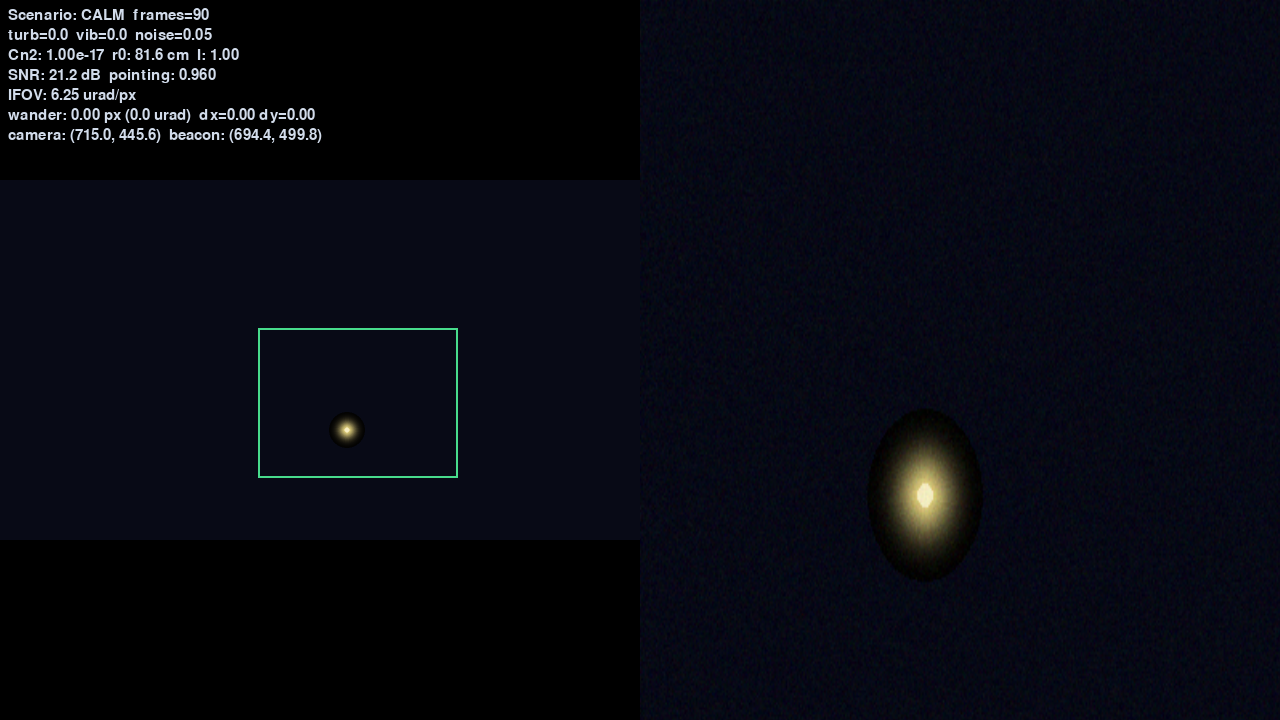
\includegraphics[width=0.92\textwidth]{physics_calm.png}
\caption{Representative GUI layout under the Calm scenario (overview, FOV, HUD).}
\label{fig:gui}
\end{figure}

\subsection{Main view (viewport)}
\begin{table}[H]
\centering
\caption{Viewport regions}
\label{tab:viewport}
\small
\begin{tabular}{@{}p{3.2cm}p{10.5cm}@{}}
\toprule
\textbf{Region} & \textbf{Content} \\
\midrule
Scene overview & Full virtual world with moving beacon(s); green box marks camera FOV. \\
Camera FOV panel & Disturbed live crop seen by the detector (turbulence, vibration, noise, weather). \\
HUD (typically TL) & Camera boresight, detector mode, FPS, tracking error (px + µrad), lock state. \\
Link Readiness gauge & Score $S\in[0,1]$; green $\ge0.7$, yellow mid-band, red low / LOST. \\
\bottomrule
\end{tabular}
\end{table}

\subsection{Overlays on the camera feed}
\begin{table}[H]
\centering
\caption{Detection / tracking overlays}
\label{tab:overlays}
\small
\begin{tabular}{@{}ll@{}}
\toprule
\textbf{Symbol} & \textbf{Meaning} \\
\midrule
Cyan crosshair & Raw detector measurement \\
Magenta marker & Kalman filter estimate (camera is driven by this) \\
Search path (overview) & Re-acquisition waypoints when tracking state is LOST \\
\bottomrule
\end{tabular}
\end{table}

\subsection{Control panel (bottom strip)}
Mouse-driven controls (Physics window; PS window scales similarly):

\begin{table}[H]
\centering
\caption{Control panel widgets}
\label{tab:panel}
\small
\begin{tabular}{@{}p{3.4cm}p{10.3cm}@{}}
\toprule
\textbf{Control} & \textbf{Function} \\
\midrule
Cn2 proxy slider & Turbulence strength $s\in[0,10]$ (log-mapped to Cn$^2$). \\
Vibration slider & Platform tip/tilt amplitude. \\
Sensor Noise slider & Camera noise level (0--1 class). \\
Slew Rate slider & Camera plant slew authority (px/s class; profile-dependent). \\
Trajectory buttons & Linear / Circular / Random / Fig-8. \\
Detector buttons & Classical (threshold centroid) / AI (hybrid fusion path). \\
Beacons buttons & 1 or 2 beacons (second beacon acts as distractor). \\
Scenario buttons & Calm / UAV / Stress one-click presets. \\
\bottomrule
\end{tabular}
\end{table}

\begin{figure}[H]
\centering
\begin{subfigure}{0.48\textwidth}
  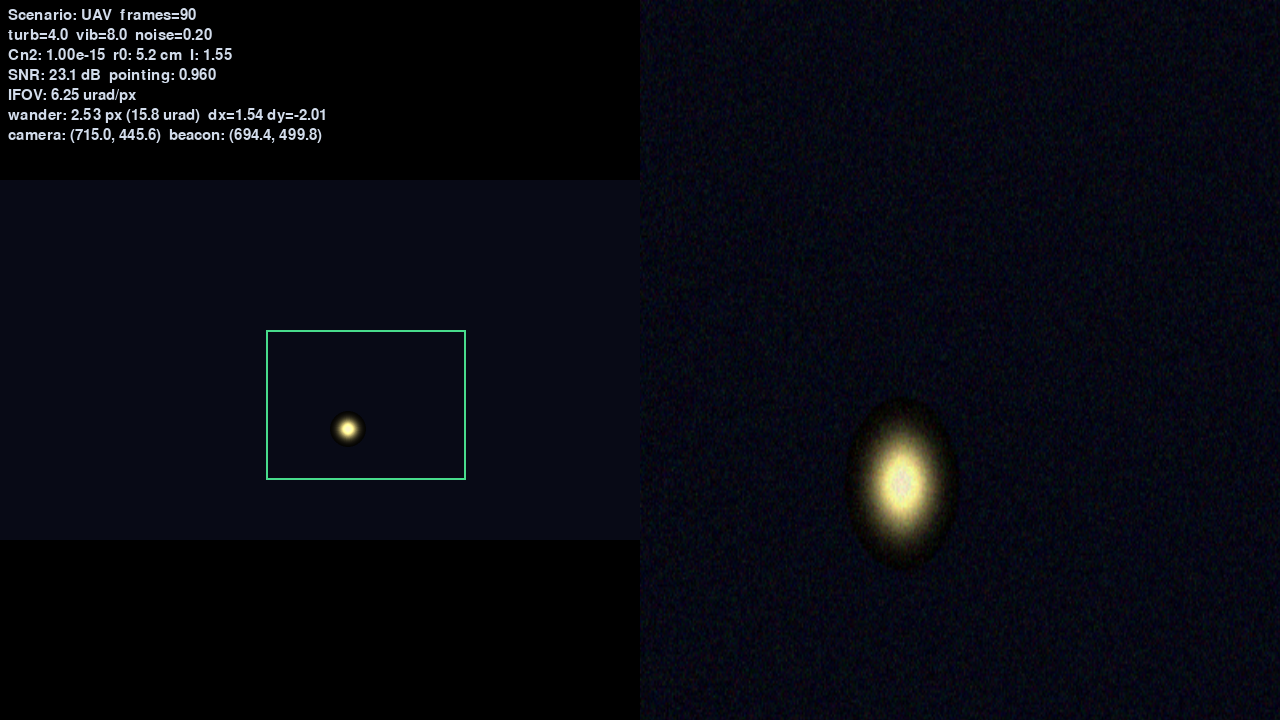
\includegraphics[width=\linewidth]{physics_uav.png}
  \caption{UAV preset}
\end{subfigure}
\hfill
\begin{subfigure}{0.48\textwidth}
  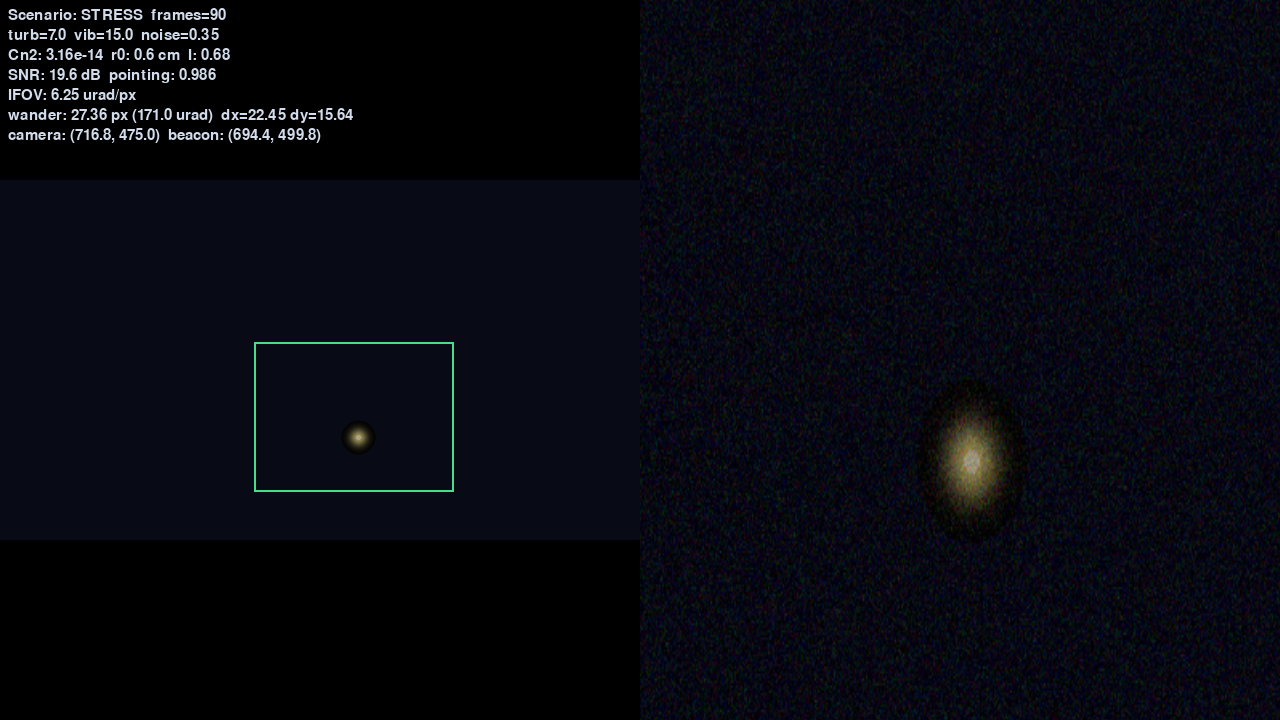
\includegraphics[width=\linewidth]{physics_stress.png}
  \caption{Stress preset}
\end{subfigure}
\caption{GUI under mobile and stress disturbance presets.}
\label{fig:presets}
\end{figure}

%% ============================================================
\section{Application Operation}
%% ============================================================

\subsection{Typical demo flow (recommended)}
\begin{enumerate}
  \item Launch \texttt{python main.py}.
  \item Click \textbf{Calm} (or press F1). Confirm LOCKED and low residual on HUD.
  \item Switch to \textbf{UAV} (F2). Observe lock retention under moderate channel + vibration.
  \item Switch to \textbf{Stress} (F3). Expect possible LOST $\rightarrow$ raster re-acquisition $\rightarrow$ re-lock.
  \item Press \textbf{L} to blind the detector briefly and demonstrate re-acquisition deliberately.
  \item Press \textbf{T} to toggle Classical $\leftrightarrow$ AI (hybrid) and compare behavior.
  \item Optionally press \textbf{B} for two beacons; press \textbf{4} for figure-of-eight motion.
  \item Quit with ESC; open the generated CSV in Streamlit (Section~\ref{sec:report}).
\end{enumerate}

\begin{figure}[H]
\centering
\begin{subfigure}{0.48\textwidth}
  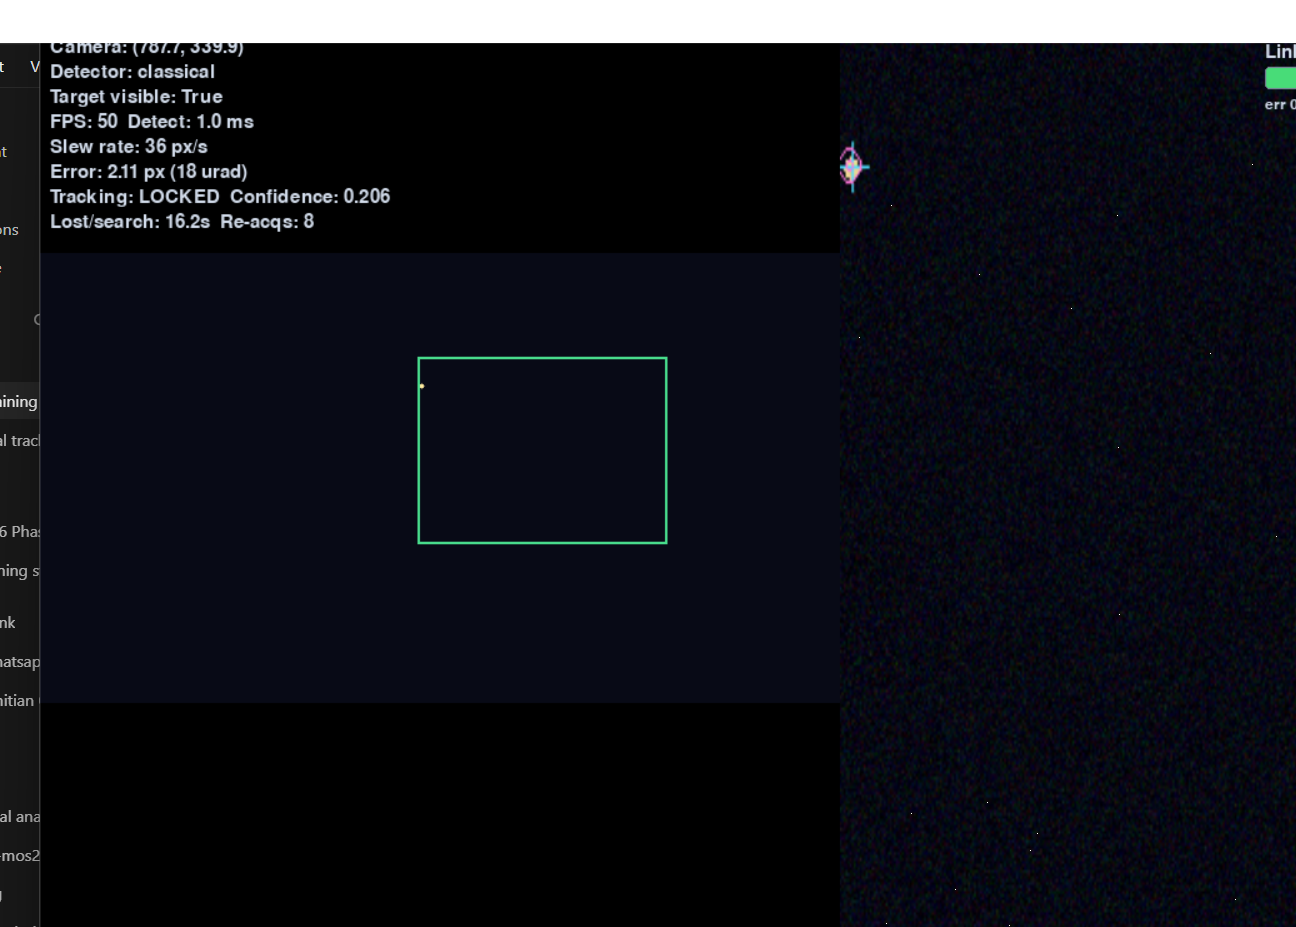
\includegraphics[width=\linewidth]{reacquire.png}
  \caption{Re-acquisition after lock loss}
\end{subfigure}
\hfill
\begin{subfigure}{0.48\textwidth}
  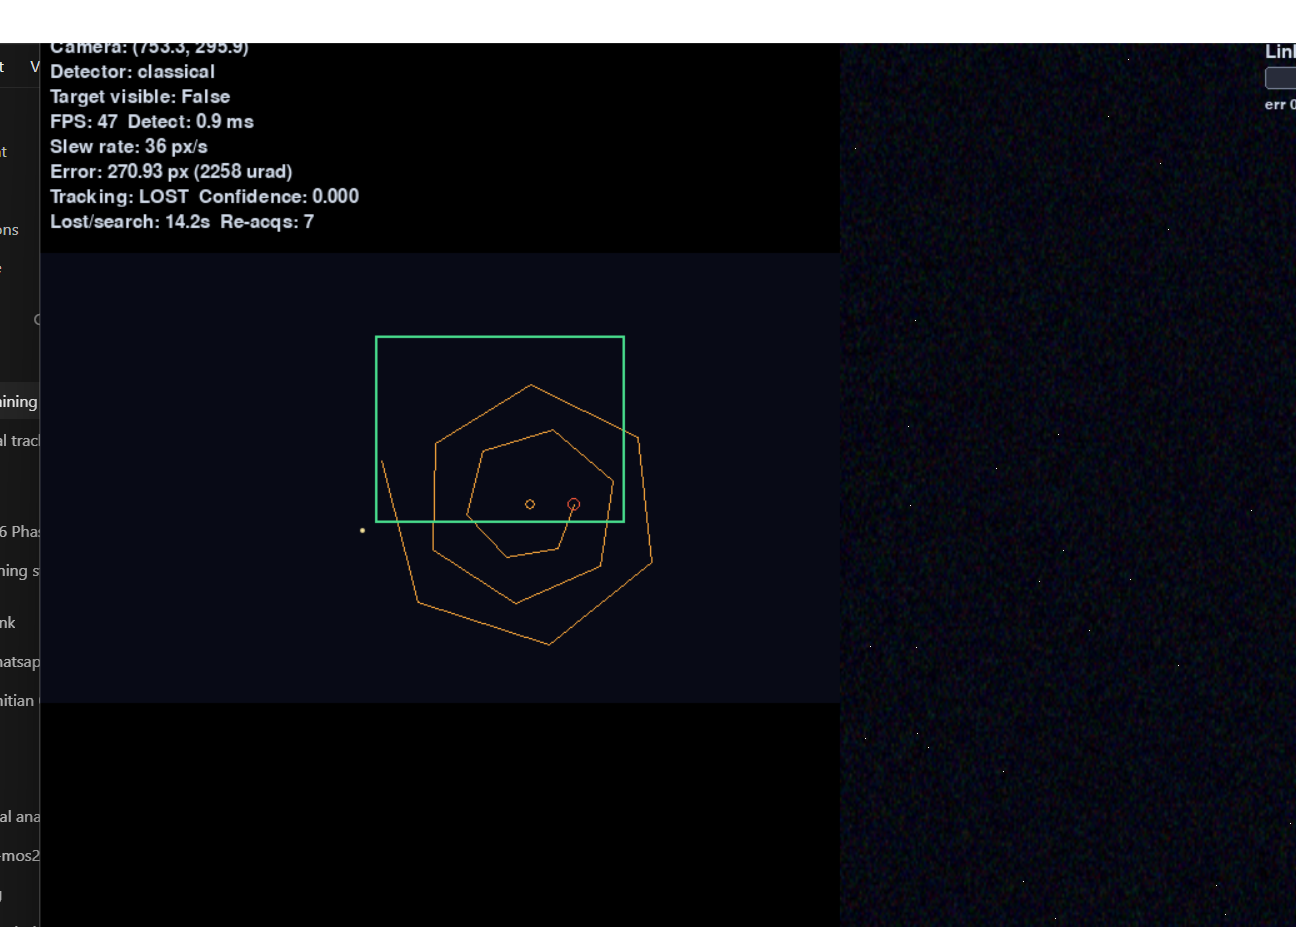
\includegraphics[width=\linewidth]{after_blind.png}
  \caption{After forced detector blind (\texttt{L})}
\end{subfigure}
\caption{Operational captures for lock-loss and recovery demos.}
\label{fig:ops}
\end{figure}

\subsection{Tracking states}
\begin{table}[H]
\centering
\caption{Tracker state machine (visible on HUD / logs)}
\begin{tabular}{@{}ll@{}}
\toprule
\textbf{State} & \textbf{Meaning} \\
\midrule
LOCKED & Valid detection accepted this frame \\
COASTING & Temporary misses; filter coasts on prediction \\
LOST & Extended misses; raster re-acquisition owns the slew \\
\bottomrule
\end{tabular}
\end{table}

\subsection{Fine pointing handoff (automatic)}
When Link Readiness $S\ge0.7$, tracking is LOCKED, and residual stays inside the capture cone for consecutive frames, the Fine mock (4-QD / FSM) may engage.
It exits with hysteresis when $S\le0.55$ or residual grows.
This is a demonstration of coarse-to-fine handoff, not a flight FSM calibration.

%% ============================================================
\section{Parameter Configuration}
%% ============================================================

\subsection{Scenario presets}
\begin{table}[H]
\centering
\caption{Built-in disturbance presets}
\label{tab:scenarios}
\small
\begin{tabular}{@{}lrrrll@{}}
\toprule
Preset & Turb & Vib & Noise & Slew & Trajectory \\
\midrule
Calm (F1) & 0 & 0 & 0.05 & 90 & Circular \\
UAV (F2) & 4 & 8 & 0.2 & 90 & Circular \\
Stress (F3) & 7 & 15 & 0.35 & 120 & Random \\
\bottomrule
\end{tabular}
\end{table}

\subsection{Live disturbance and plant parameters}
\begin{table}[H]
\centering
\caption{Configurable live parameters}
\label{tab:params}
\small
\begin{tabular}{@{}p{3.6cm}p{3.4cm}p{6.5cm}@{}}
\toprule
\textbf{Parameter} & \textbf{UI / keys} & \textbf{Notes} \\
\midrule
Turbulence (Cn2 proxy) & Slider; Q/A & Maps to atmospheric wander/scintillation. \\
Vibration & Slider; W/S & Platform tip/tilt on FOV. \\
Sensor noise & Slider; E/D & Image grain; interacts with weather. \\
Slew rate & Slider & Camera plant authority. \\
Trajectory & Buttons; 1--4 & Includes PS-required figure-8. \\
Detector mode & Buttons; T & Classical vs AI (hybrid). \\
Beacon count & Buttons; B & 1 or 2. \\
Noise type & N & Legacy / Gaussian / salt--pepper / Poisson. \\
Weather grade & M & Clear $\rightarrow$ Haze $\rightarrow$ Fog $\rightarrow$ Rain $\rightarrow$ Low light. \\
\bottomrule
\end{tabular}
\end{table}

\subsection{Keyboard reference}
\begin{table}[H]
\centering
\caption{Complete keyboard shortcuts}
\label{tab:keys}
\small
\begin{tabular}{@{}cl@{}}
\toprule
\textbf{Key} & \textbf{Action} \\
\midrule
1 / 2 / 3 / 4 & Trajectory: linear / circular / random / figure-8 \\
Q / A & Turbulence + / $-$ \\
W / S & Vibration + / $-$ \\
E / D & Sensor noise + / $-$ \\
T & Toggle Classical $\leftrightarrow$ AI \\
B & Toggle 1 $\leftrightarrow$ 2 beacons \\
N & Cycle noise type \\
M & Cycle weather preset \\
L & Blind detector for a fixed frame count (force re-acq test) \\
F1 / F2 / F3 & Calm / UAV / Stress \\
ESC & Quit application \\
\bottomrule
\end{tabular}
\end{table}

%% ============================================================
\section{Logging and Performance Report}
\label{sec:report}
%% ============================================================

\subsection{Automatic logs}
Each interactive session writes:
\begin{itemize}
  \item \texttt{logs/run\_YYYY-MM-DD\_HHMM.csv} --- per-frame / session metrics;
  \item \texttt{logs/run\_*.summary.json} --- run sheet (acquisition time, lock \%, FPS, errors, etc.).
\end{itemize}

\subsection{Streamlit report}
\begin{lstlisting}
streamlit run report.py
\end{lstlisting}
\begin{enumerate}
  \item Select a CSV from \texttt{logs/}.
  \item Optionally enable comparison of two runs (Classical vs AI).
  \item Download text or PDF performance report for judges.
\end{enumerate}

\subsection{Matched Classical vs AI benchmark}
\begin{lstlisting}
python scripts/run_comparison.py --duration 60
\end{lstlisting}
Produces matched-seed CSV pairs under \texttt{logs/} for fair detector comparison.

\subsection{Benchmark-2 (judge MP4, PTZ bypass)}
\begin{lstlisting}
python scripts/generate_ps_test_video.py
python scripts/benchmark_video.py --video logs/benchmark2/ps_sample.mp4 --gt logs/benchmark2/ps_sample_gt.csv
\end{lstlisting}
Use the same script on judge-provided videos; set \texttt{--detector ai} when needed.
Outputs include centroid CSV and a summary JSON with \texttt{ptz\_bypassed: true}.

\subsection{Other evaluation utilities}
\begin{itemize}
  \item Acquisition Monte Carlo: \path{scripts/monte_carlo_acquisition.py}
  \item Detection Pd/Pfa: \path{scripts/evaluate_detection.py}
  \item Demo video capture: \path{scripts/record_demo_video.py}
\end{itemize}

%% ============================================================
\section{Troubleshooting}
%% ============================================================

\begin{table}[H]
\centering
\caption{Common issues}
\label{tab:trouble}
\small
\begin{tabular}{@{}p{4.8cm}p{8.8cm}@{}}
\toprule
\textbf{Symptom} & \textbf{Action} \\
\midrule
AI mode unavailable / reverts & Ensure \texttt{weights/beacon\_yolov8n.pt} exists; retrain if missing. \\
Low FPS with AI on CPU & Expected; use Classical for smooth live demos or enable CUDA. \\
Black / empty FOV & Reduce Stress disturbances; wait for re-acquisition; check beacon in overview. \\
No log files & Run longer than $\sim$1\,s before ESC; check write permission on \texttt{logs/}. \\
Import / package errors & Activate \texttt{.venv} and re-run \texttt{pip install -r requirements.txt}. \\
PS window too large & Use a high-resolution display or stay on Physics profile for demos. \\
\bottomrule
\end{tabular}
\end{table}

%% ============================================================
\section{Related Documents}
%% ============================================================

\begin{itemize}
  \item Technical report (algorithms, architecture, results): \path{docs/sih_technical_report.pdf}
  \item Compliance notes: \path{docs/sih_compliance.md}, \path{docs/ps_compliance_gaps.md}
  \item Markdown quick reference (this manual's source twin): \path{docs/user_manual.md}
\end{itemize}

\vspace{1.2em}
\noindent\textit{End of User Manual --- BeamLock / Team Cadets / SIH26169.}

\end{document}
